\section{Overview}

The Students\&Companies (S\&C) platform is designed as a client-server application, where the term \textit{client} refers to the users of the system: students, companies, and universities. We have chosen a \textit{fat client} approach to provide a highly interactive, app-like experience, enabling responsive and rich functionality directly in the browser. This approach also reduces server load by offloading some processing to the client side, enhancing scalability.

Users interact with the system through a Single Page Application (SPA), a desktop web application that serves as the primary user interface for accessing platform features. The SPA allows for seamless navigation and interaction, providing a user experience similar to that of a native application. By managing application state on the client side, the SPA minimizes page reloads, enhancing usability and responsiveness.

On the backend, we have followed a \textit{monolithic server} approach. This choice simplifies the overall system architecture by consolidating functionality into a single codebase, which can facilitate easier development, deployment, and maintenance. Although monolithic, the server is structured into multiple controllers and services, each responsible for specific areas, such as authentication, internship management, profile handling, and recommendations. This modular organization within the monolith ensures that each component is cohesive and manageable while maintaining performance and consistency.

To facilitate the communication between the client and the server, we are also including the usage of a web server. This web server would act as an intermediary, handling client requests and routing them to the backend. Including a web server supports secure connections, and serve for load balancing and scalability enhancements.

To support database, storage, and email services, we are using a cloud provider infrastructure. Specifically, we utilize Amazon Web Services (AWS) with Amazon RDS for the database, Amazon S3 for file storage, and Amazon SES for email notifications.

\begin{figure}[!ht]
    \centering
    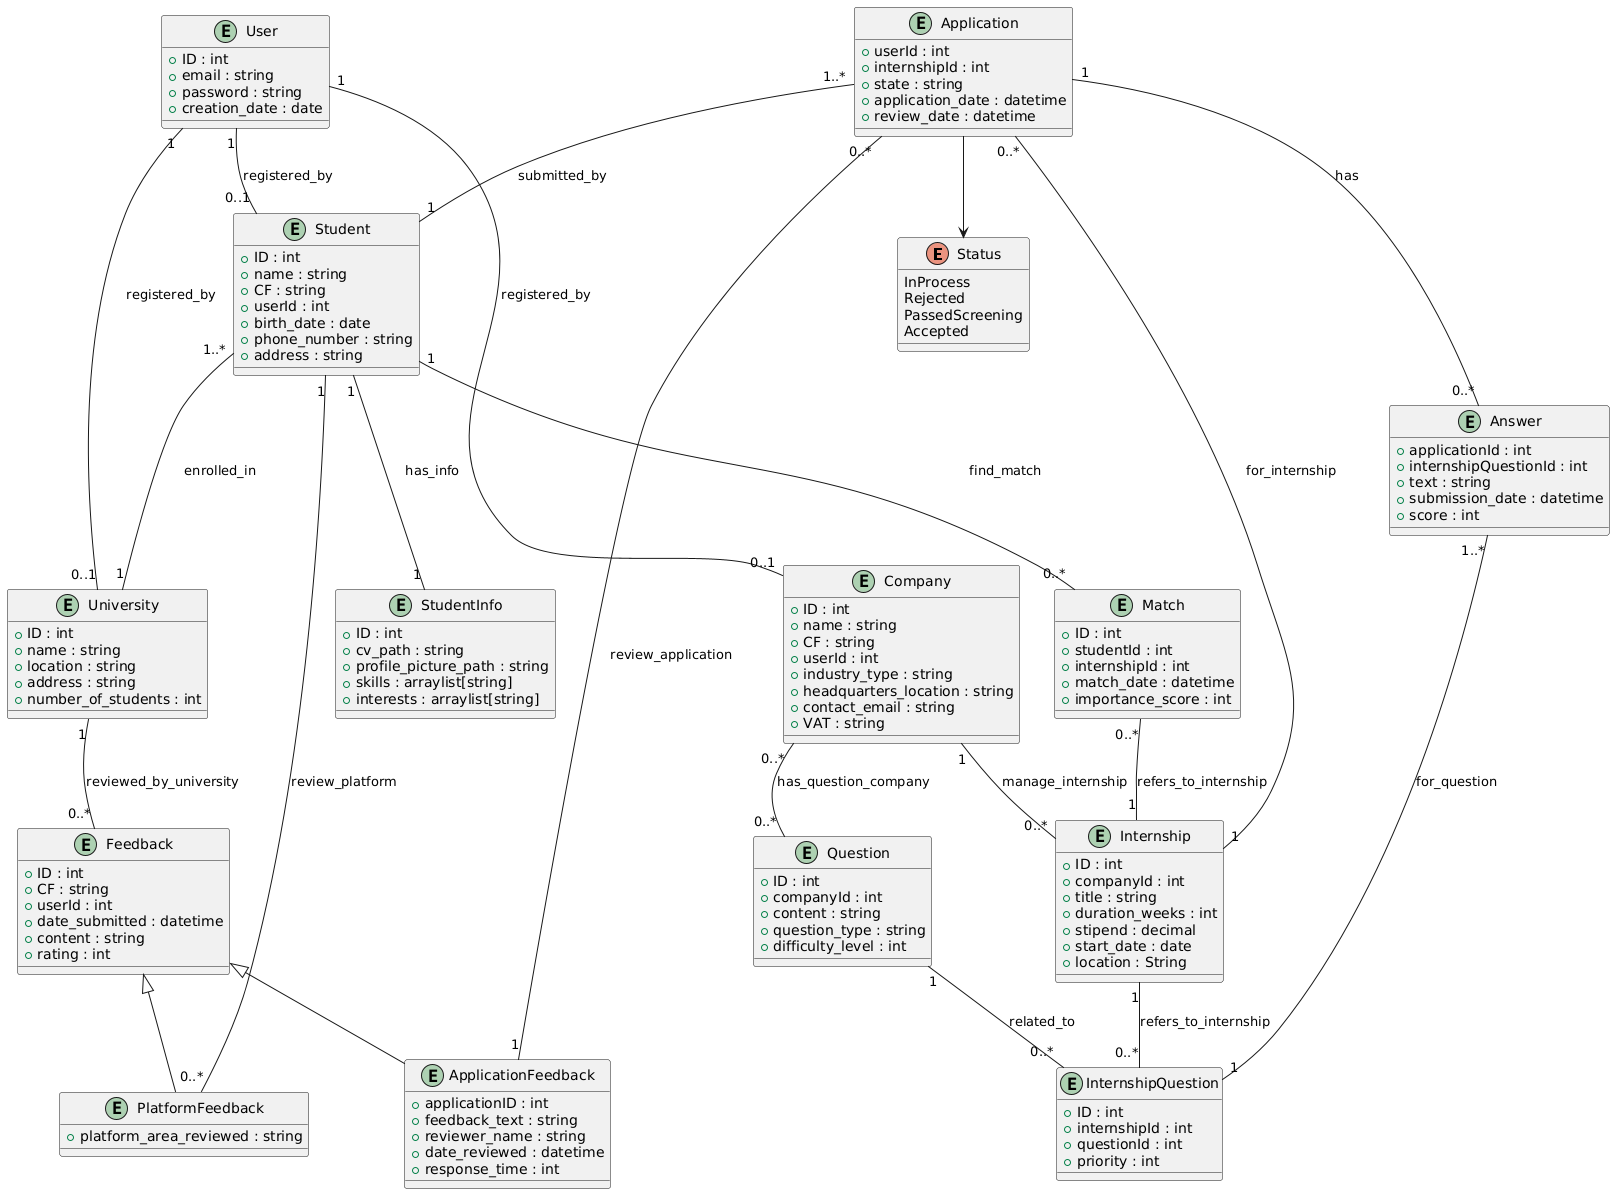
\includegraphics[scale=0.33]{Images/ImagesDD/class_diagram.png}
    \caption{Class diagram}
\end{figure}


\newpage

\section{Component view}

\subsection{Client Components}
The principal component of the client side is the Web-App, which the user will interact with.

\subsection{Server Components}

In the server side, resides the principal components such as the controller used to manage the HTTP request sent by the user.

\begin{itemize}
\item \textbf{Internship}: Handles the logic related to managing internships, including creating, updating, and tracking internship opportunities. It allows administrators and companies to post internship positions and lets students apply, track, and view their application statuses.

\item \textbf{Student}: Manages all student-related data, including profile creation, academic details, and progress tracking. It allows students to update their profiles and view their application history, while administrators can monitor student progress and make updates as needed.

\item \textbf{Feedback}: Implements the system for collecting and managing feedback from students, companies, and administrators. This component allows participants to submit feedback on internship experiences, and administrators can review and analyze this feedback to improve the program.

\item \textbf{Company}: Responsible for managing company accounts and profiles, as well as facilitating company interactions with students and internships. It allows companies to create profiles, post internship opportunities, and review student applications, making the hiring and feedback process streamlined and accessible.


\item \textbf{Authentication Controller}:
The Authentication Controller handles all processes related to user authentication, such as logging in, logging out, session validation, and password management.
\end{itemize}

\subsection{Data Component}

We use a relational database hosted on AWS to securely manage and organize structured data for the application. AWS’s managed RDS service offers high availability, automated backups, and scalability, ensuring reliable data storage and quick access for all server components. This setup allows us to maintain relational integrity, enforce data consistency, and easily scale as our data requirements grow.
\section{Deployment view}

The frontend is a SPA implemented with the React framework. The website can be visited from any modern web browser, such as Google Chrome, Mozilla Firefox or Microsoft Edge. \\ \\
Clients can be any desktop device that can run the previous browsers, such as computers with Windows, Linux or macOS.
The website is served by a CDN like Amazon CloudFront.
Using a CDN greatly enhances performance by caching static assets on globally distributed servers, ensuring users access content from locations closest to them for faster load times and reduced latency. \\ \\
The backend of the platform is powered by an ASP.NET Core server, deployed within a Kubernetes cluster that orchestrates and manages the containerized environment. This setup ensures that the backend is scalable, resilient, and highly available, with Kubernetes automating the deployment, scaling, and management of application pods. NGINX is used within the cluster as an Ingress Controller, handling incoming traffic, SSL termination, and advanced routing rules. Kubernetes performs horizontal scaling by automatically deploying new pods during traffic surges to maintain seamless performance.\\ \\
The ASP.NET Core application communicates with AWS services like RDS for database and S3 for storage. Continuous integration and deployment pipelines facilitate automated updates, pushing new Docker images to the cluster and enabling rolling updates with minimal downtime.\\ \\
This integration of Kubernetes and NGINX ensures that the backend infrastructure is robust and adaptable, capable of handling large volumes of requests while providing efficient load distribution and reliability.

\todo{add diagram}
\newpage


\section{Runtime view}
The following function (2.2) for simplicity is represented in another diagram, but it is meant to be intended as an action that happens before all the other diagrams.
\vspace{5mm}

\begin{figure}[ht!]
    \centering
    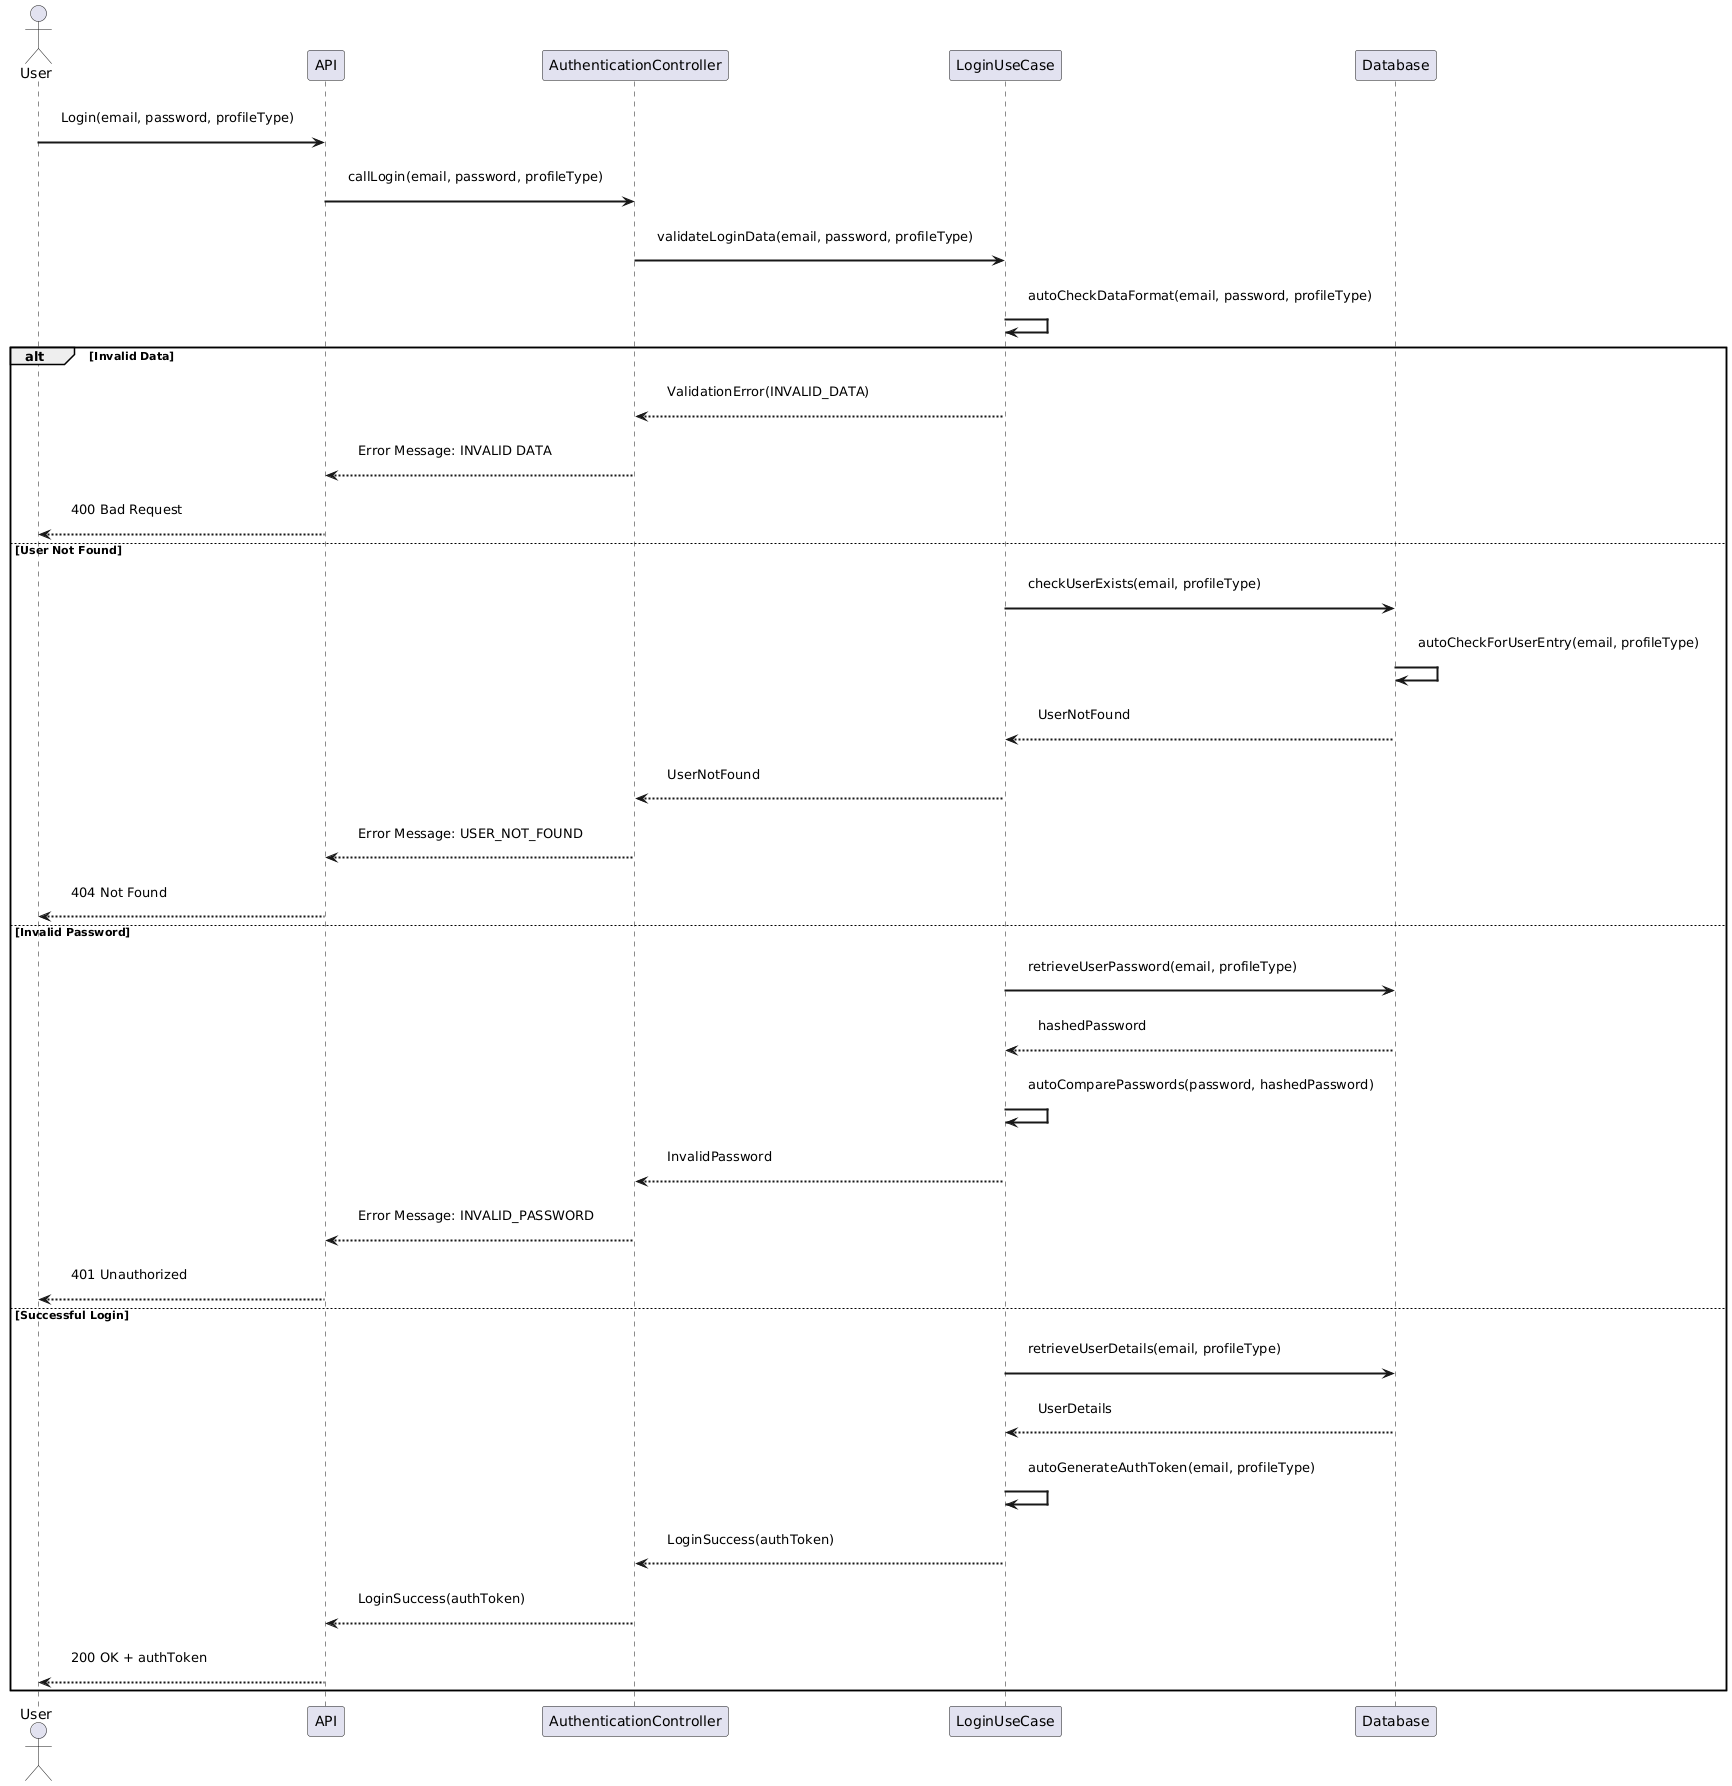
\includegraphics[scale=0.80]{Images/ImagesSequenceDiagram/LoginAuthentication.png}
    \caption{User (Student, Company or University) Authentication process}
\end{figure}

\newpage

\begin{figure}[ht!]
    \centering
    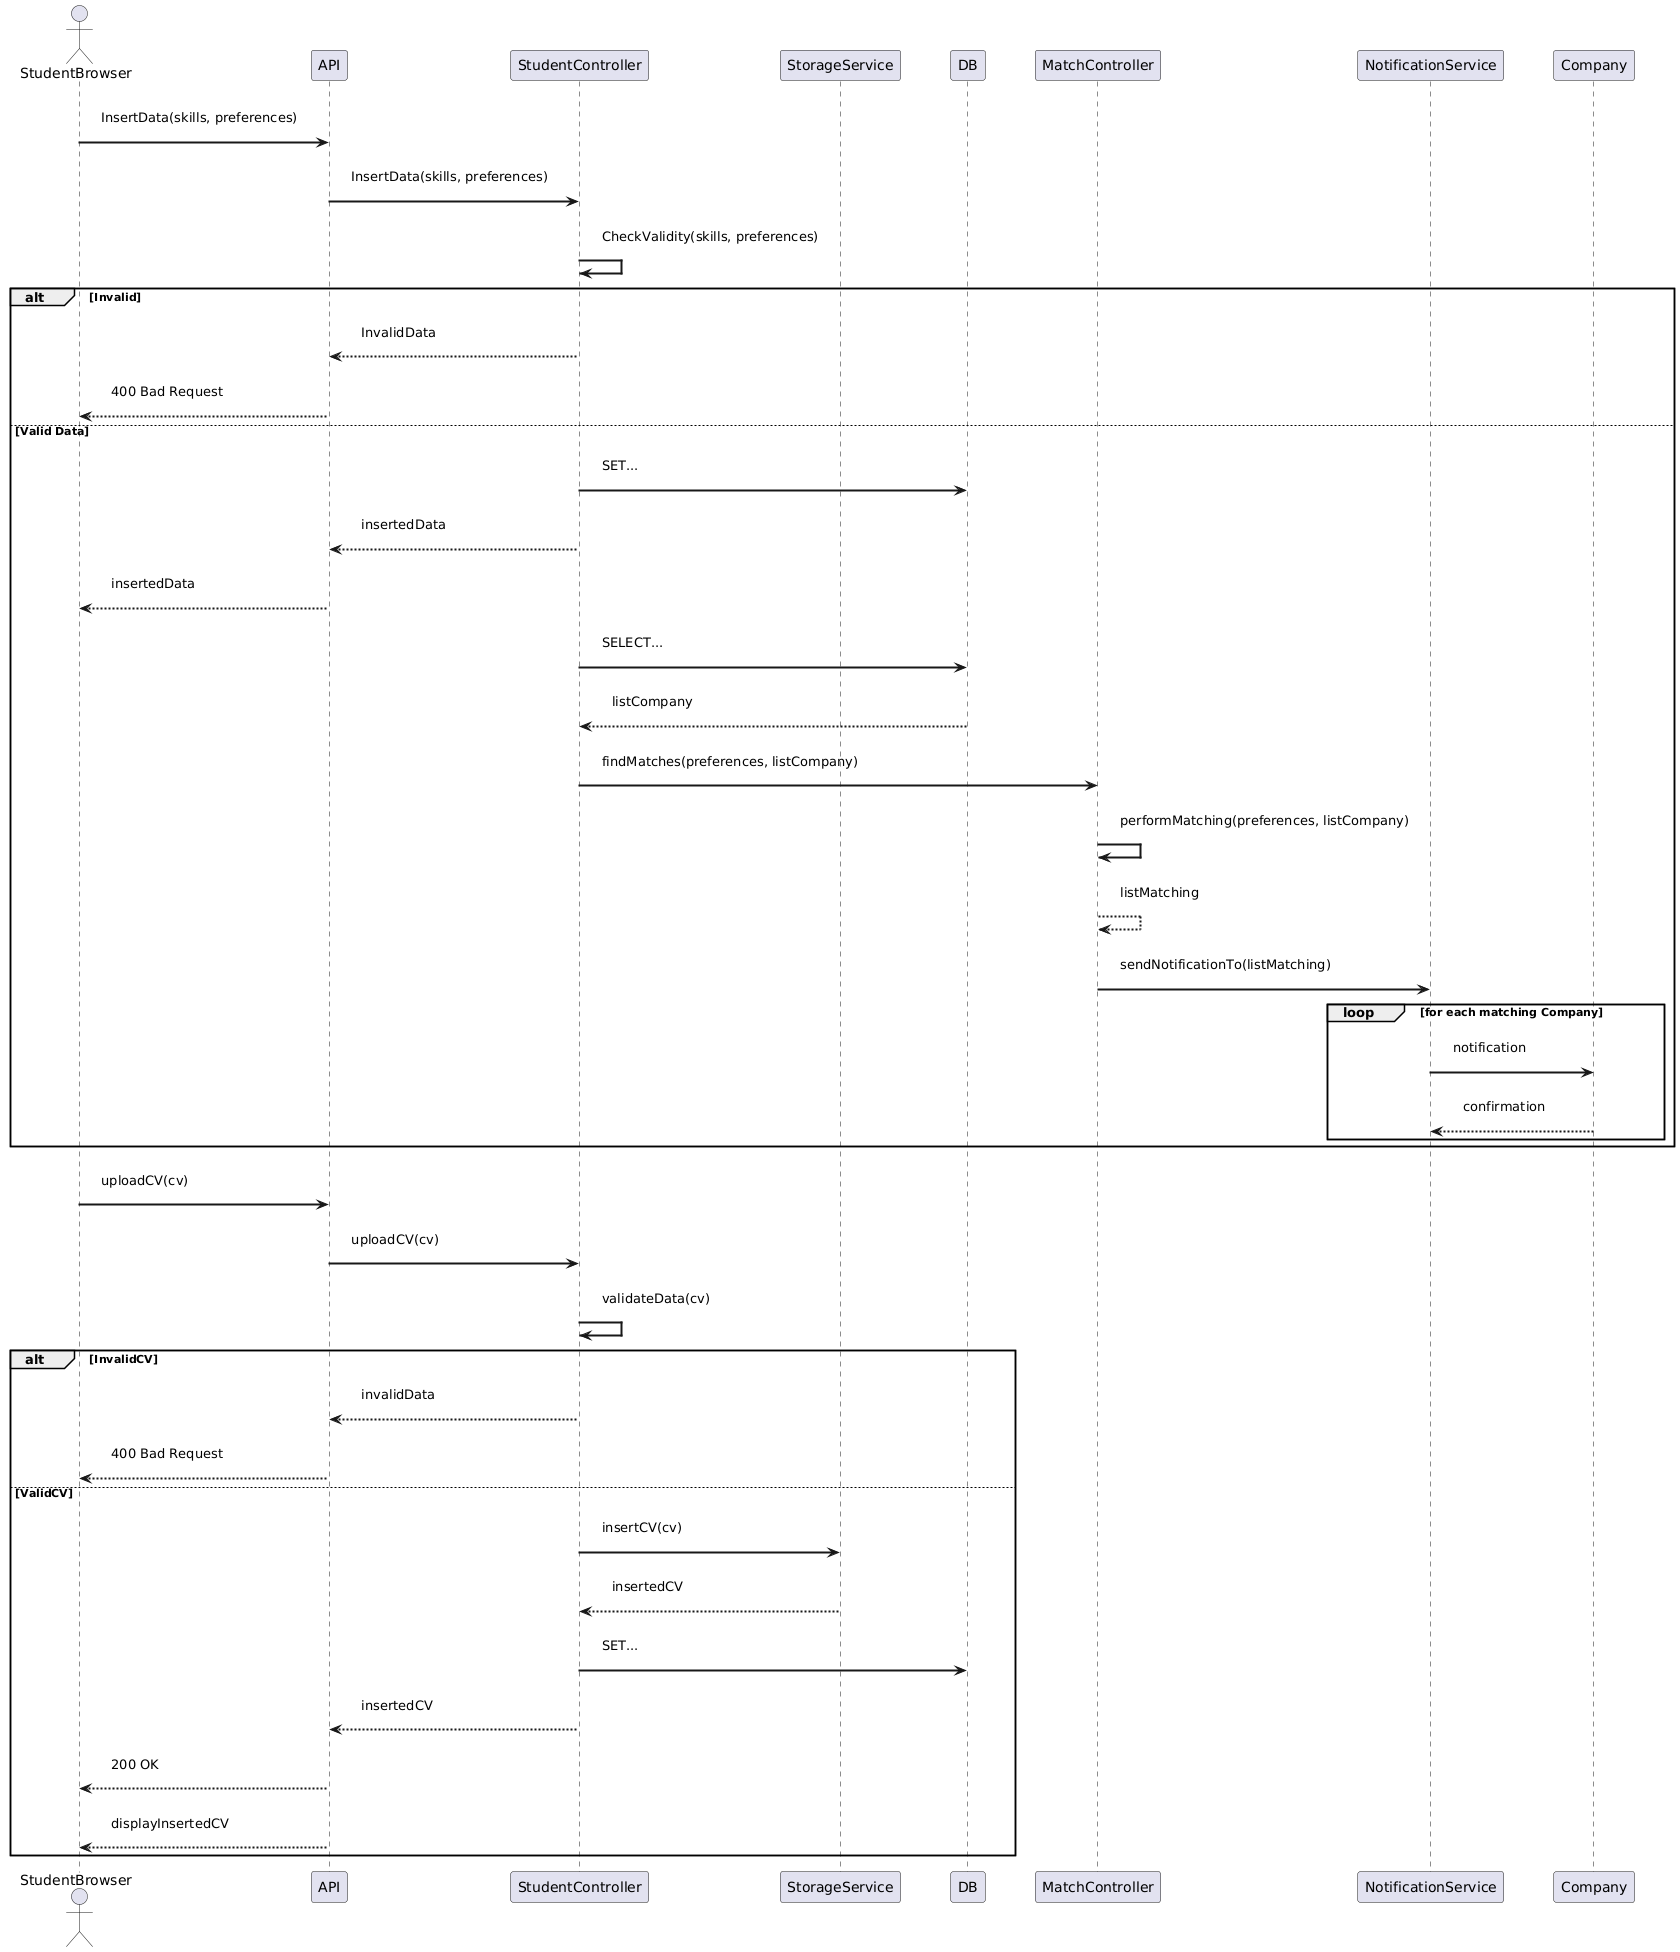
\includegraphics[scale=0.3]{Images/ImagesSequenceDiagram/StudentUploadCV.png}
    \caption{Student inserts CV and data}
\end{figure}

\newpage

\begin{figure}[ht!]
    \centering
    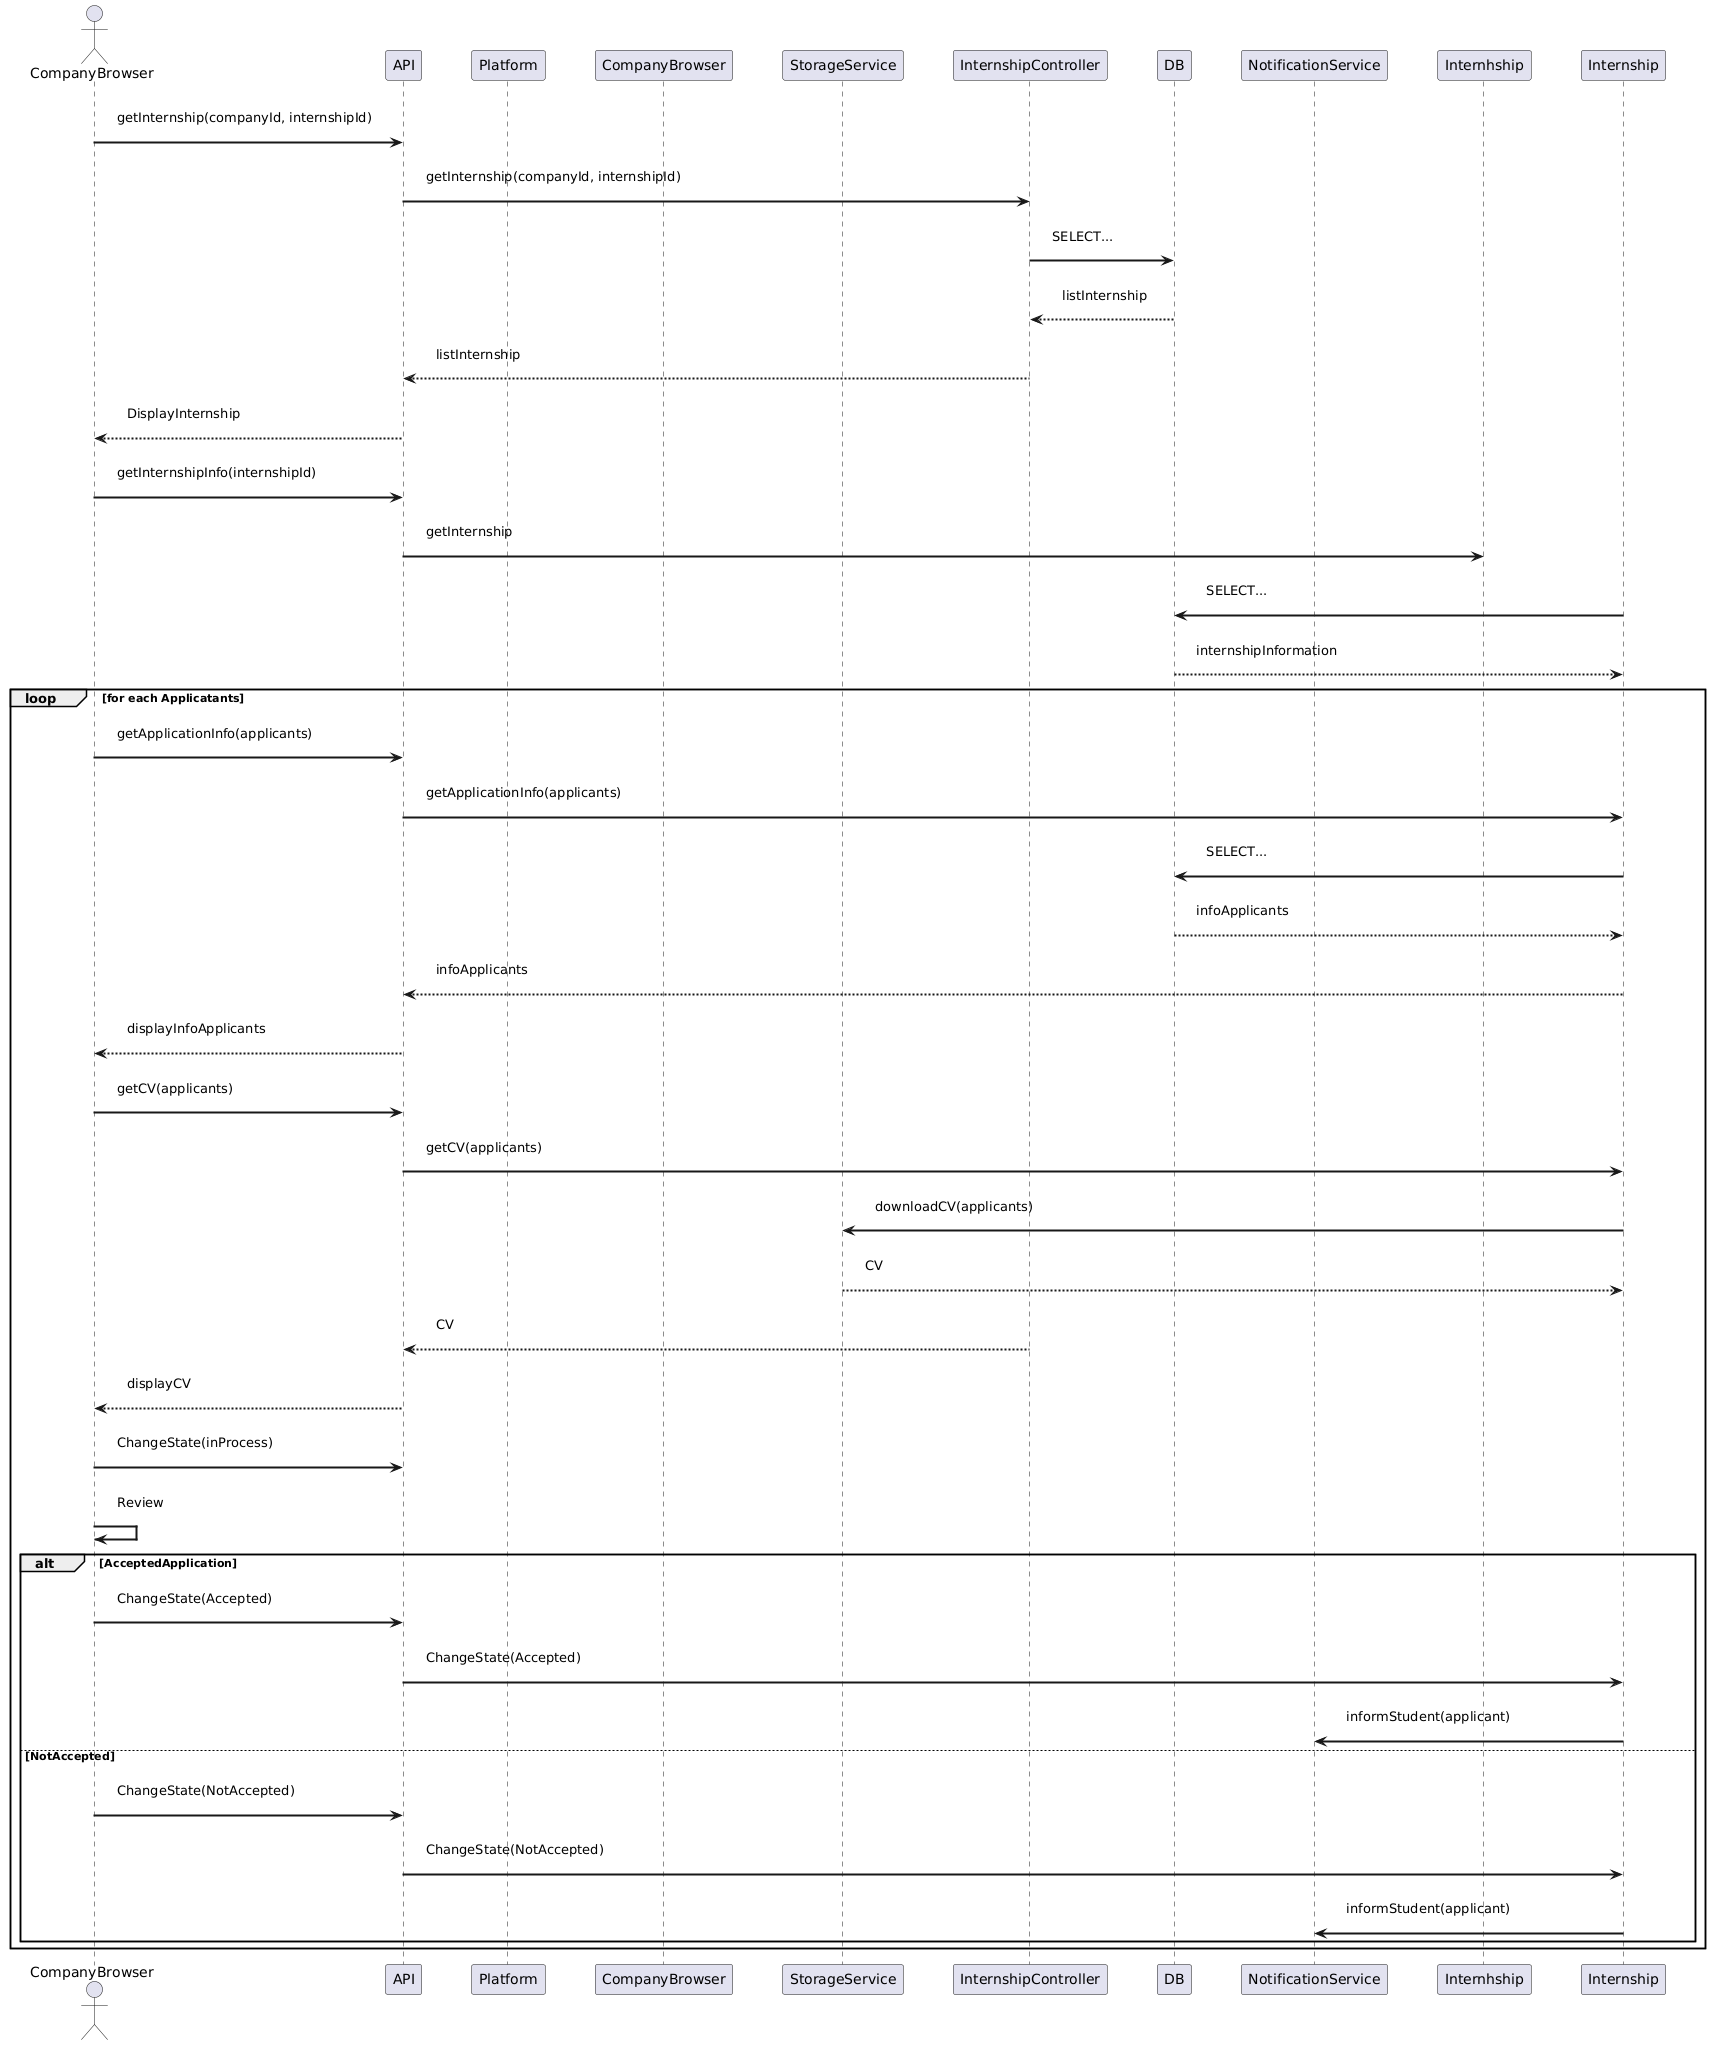
\includegraphics[scale=0.25]{Images/ImagesSequenceDiagram/CompanyReviewApplication.png}
    \caption{Company reviews application}
\end{figure}

\newpage

\begin{figure}[ht!]
    \centering
    \includegraphics[scale=0.4]{Images/ImagesSequenceDiagram/StudentsQuestions.png}
    \caption{Student answers questions}
\end{figure}

\newpage




\section{Component interfaces}

\begin{itemize}
\item \textbf{Authentication Controller}
The Authentication Controller handles all processes related to user authentication, such as logging in, logging out, session validation, and password management.

\begin{itemize}
    \item \textbf{login(username: String, password: String): String?} – Authenticates a user (student or company) by validating credentials. If successful, returns an \textit{authToken}.
    \item \textbf{logout(authToken: String): void} – Logs out the user associated with the provided \textit{authToken}, ending their session.
    \item \textbf{validateToken(authToken: String): Bool} – Checks if the provided \textit{authToken} is valid and active, returning \textit{true} if valid and \textit{false} otherwise.
    \item \textbf{refreshToken(authToken: String): String?} – Extends the session duration by generating a new \textit{authToken} if the current one is valid, returning the new token.
    \item \textbf{resetPasswordRequest(email: String): void} – Sends a password reset link to the provided email, allowing users to initiate the password reset process.
    \item \textbf{resetPassword(token: String, newPassword: String): Bool} – Validates the reset token sent to the user's email and updates the password if the token is valid. Returns \textit{true} upon success.
    \item \textbf{registerUser(userData: User): ID} – Registers a new user (student or company) by saving the provided user data and returns the unique \textit{userId}.
\end{itemize}

\item \textbf{Internship}

\begin{itemize}
    \item \textbf{createInternship(companyId: ID, internshipData: Internship): ID} – Allows a company to create a new internship posting, returning the ID of the new internship.
    \item \textbf{updateInternship(internshipId: ID, updatedData: Internship): void} – Updates an existing internship posting with new information provided by the company.
    \item \textbf{deleteInternship(internshipId: ID): void} – Deletes an internship listing, making it inactive or removing it from the view.
    \item \textbf{getInternshipDetails(internshipId: ID): Internship} – Retrieves detailed information about a specific internship by its ID.
    \item \textbf{listAllInternships(filters: InternshipFilters): List<Internship>} – Returns a list of internships based on filters (e.g., location, industry, duration).
    \item \textbf{applyToInternship(studentId: ID, internshipId: ID, applicationData: Application): ID} – Allows a student to apply to an internship and returns an application ID.
    \item \textbf{getApplications(internshipId: ID): List<Application>} – Retrieves all applications for a specific internship, visible to the company that posted it.
    \item \textbf{getApplicationStatus(applicationId: ID): ApplicationStatus} – Returns the current status of a specific application for tracking purposes.
\end{itemize}
\todo{Add answer controller for a specific internship}
\item \textbf{Student Controller}
The Student Controller manages requests related to student profiles, such as updates and viewing application history.

\begin{itemize}
    \item \textbf{createStudentProfile(studentData: Student): ID} – Creates a new student profile and returns the unique student ID.
    \item \textbf{updateStudentProfile(studentId: ID, updatedData: Student): void} – Allows a student to update their profile with new information, such as contact details or academic information.
    \item \textbf{getStudentProfile(studentId: ID): Student} – Retrieves the profile details for a specific student.
    \item \textbf{listStudentApplications(studentId: ID): List<Application>} – Returns the history of internship applications made by the student.
    \item \textbf{viewSavedInternships(studentId: ID): List<Internship>} – Lists all internships that the student has saved for future consideration.
    \item \textbf{saveInternship(studentId: ID, internshipId: ID): void} – Allows a student to save an internship to their saved list.
\end{itemize}

\item \textbf{Feedback Controller}
The Feedback Controller manages operations for collecting and handling feedback within the system.

\begin{itemize}
    \item \textbf{submitFeedback(userId: ID, internshipId: ID, feedbackData: Feedback): void} – Allows a user (student or company) to submit feedback on an internship or application experience.
    \item \textbf{getFeedbackForInternship(internshipId: ID): List<Feedback>} – Retrieves all feedback associated with a specific internship, useful for administrators to monitor feedback trends.
    \item \textbf{getFeedbackForStudent(studentId: ID): List<Feedback>} – Retrieves feedback given to or by a student, allowing administrators to track individual experiences.
    \item \textbf{analyzeFeedbackForReport(reportCriteria: FeedbackCriteria): FeedbackReport} – Generates a report based on specified feedback criteria, enabling analysis of trends and areas for improvement.
\end{itemize}

\item \textbf{Company Controller}
The Company Controller is responsible for managing company accounts and interaction with internship postings and applications.

\begin{itemize}
    \item \textbf{createCompanyProfile(companyData: Company): ID} – Creates a new company profile and returns the company ID.
    \item \textbf{updateCompanyProfile(companyId: ID, updatedData: Company): void} – Allows a company to update its profile information, such as contact details or industry.
    \item \textbf{getCompanyProfile(companyId: ID): Company} – Retrieves profile information for a specific company.
    \item \textbf{listCompanyInternships(companyId: ID): List<Internship>} – Lists all internships posted by the company.
    \item \textbf{reviewApplications(companyId: ID, internshipId: ID): List<Application>} – Retrieves a list of applications for a specific internship posted by the company.
    \item \textbf{acceptApplication(companyId: ID, applicationId: ID): void} – Allows a company to accept a student application for an internship.
    \item \textbf{rejectApplication(companyId: ID, applicationId: ID): void} – Allows a company to reject a student application for an internship.
\end{itemize}
\newpage

\end{itemize}


\section{Selected architectural styles and patterns}
\textbf{Monolithic server:} 
We chose a monolithic approach for its simplicity, faster development, and easier management. It minimizes the complexities of inter-service communication and ensures consistent control, which is ideal for smaller teams or projects with limited resources. This approach also offers better performance and simpler security management, making it a practical choice for our project’s scope

\textbf{Dependency Injection:}
In both the frontend and especially the backend, we have adhered to the dependency injection pattern. This approach promotes decoupling by allowing components to depend on abstractions rather than concrete implementations, making the codebase more modular and easier to maintain. It enhances testability by enabling the injection of mock dependencies for unit testing, ensuring that components can be tested in isolation. By following this pattern, we achieve greater flexibility, as changes to implementations can be made with minimal impact on the dependent code, facilitating future enhancements and scalability.

\textbf{Modular Controller-Service:}
We have adopted a modular approach that can be described as a Controller-Service pattern. This design emphasizes separation of concerns by having controllers handle HTTP requests and delegate business logic to dedicated service classes. Services encapsulate the core business logic, making the application easier to test, maintain, and extend. This approach decouples the logic from controllers, promoting cleaner code and improved testability. The use of a service layer helps achieve better modularity, as different parts of the application can be updated or scaled independently without tightly coupling business logic and presentation logic.

\textbf{Fat client:}
Fat clients allow offering a wide variety of functionalities independent from the central server, as well as to move part of the business logic off of the server and into the clients. The main advantages it offers are greater decoupling of frontend and backend as well as a better interactive experience, especially in conditions where the client is on an unstable network. Additionally, with the adoption of a single-page applications, there are many cross-platform frameworks which allow to reuse code partially or entirely on multiple platforms. The single-page web application can also be served by a dedicated static web server, as all its interactivity is implemented client-side, further reducing the burden on the server by delegating its serving to a CDN, which is highly optimized for
this specific use case.

\textbf{REST API:}
An architectural style defined on top of HTTP centered around the definition of a standardized set of stateless operations. Its main advantages are its simplicity, its use of widely adopted standards which facilitate adoption, and its ease of scalability given by its stateless nature. It allows to have a single API interface against which a heterogeneous set of clients can make requests.

\textbf{Component-based architecture:}
In the frontend, we have focused on a component-based architecture. This approach structures the application as a collection of reusable and self-contained components, each managing its logic, rendering, and state. By adopting this architecture, we ensure that the code is modular, making it easier to maintain, update. Reusability is a key advantage, as components can be composed and reused across different sections of the app, leading to more efficient development and consistent user interfaces.


\section{Other design decisions}

\textbf{Relational DBMS}: 
We chose to integrate a Database Management System (DBMS) into our project to ensure efficient data management, storage, and retrieval. A DBMS provides a structured and scalable way to handle large volumes of data while maintaining data integrity, consistency, and security. It allows for multi-user access, concurrent data manipulation, and facilitates complex queries that enhance the project's functionality and performance. The choice of a DBMS also supports data backup and recovery, reducing the risk of data loss and ensuring system reliability. Overall, it is an essential component for building a robust, reliable, and scalable solution